\documentclass[twocolumn,10pt]{article}

\usepackage{authblk}
\usepackage{bera}
\usepackage[utf8]{inputenc}
\usepackage{graphicx}

% TITLE
\title{Chef Classification from Recipe Text using DistilBERT Fine-Tuning}


% AUTHORS
\author{Nicholas Birch de la Calle}
\author{Gabriel [Last Name]}
\author{Javier [Last Name]}
\author{Maxence [Last Name]}
\affil{Group 2\\ Instituto Superior Técnico, Universidade de Lisboa}

\begin{document}

\maketitle

\section{Introduction}

The task of chef classification from recipe text represents an interesting natural language processing challenge that combines culinary domain knowledge with text classification. Given a recipe's name, ingredients, preparation steps, tags, and description, we aim to predict which of six chefs created it. This problem has practical applications in culinary content recommendation, authorship attribution, and understanding chef-specific cooking styles.

Our dataset consists of 2,999 labeled training recipes distributed across 6 chef classes, with a moderate class imbalance ratio of 2.17:1. We approach this as a multi-class text classification problem using transformer-based language models, specifically fine-tuning DistilBERT on concatenated recipe text fields. Our goal is to exceed the baseline accuracies of 30\% (TF-IDF on descriptions only) and 43\% (TF-IDF on all fields).

\section{Model Architecture}

We employ DistilBERT-base-uncased \cite{sanh2019distilbert}, a distilled version of BERT with 66 million parameters, 6 transformer layers, and 768-dimensional hidden states. DistilBERT retains 97\% of BERT's performance while being 40\% smaller and 60\% faster, making it well-suited for our classification task with limited computational resources.

\textbf{Input Representation:} We concatenate five text fields in priority order: recipe\_name $\rightarrow$ ingredients $\rightarrow$ tags $\rightarrow$ description $\rightarrow$ steps. This ordering protects critical identifying information (name, ingredients) from truncation, as recipe steps constitute 42\% of total tokens. Text is tokenized using DistilBERT's WordPiece tokenizer with a maximum sequence length of 512 tokens, which accommodates 98.2\% of our dataset without truncation (median: 272 tokens). DistilBERT adds a learned positional embedding vector to every token embedding, allowing the model to infer word order directly from parameters trained alongside the rest of the network (in contrast to fixed sinusoidal encodings).

\textbf{Classification Head:} The pooled [CLS] embedding first passes through dropout with $p=0.2$, then a dense projection (768 $\rightarrow$ 768) followed by a ReLU activation, a second dropout layer with the same rate, and finally a linear layer (768 $\rightarrow$ 6). The model outputs raw logits, with softmax and cross-entropy loss computed jointly during training. Figure~\ref{fig:encoder} summarises the end-to-end architecture.

\textbf{Training Strategy:} We use the AdamW optimizer with a learning rate of $2 \times 10^{-5}$, weight decay of 0.01, and linear warmup over 6\% of training steps. Training uses batch size 16 with dynamic padding (padding="longest") to minimize memory usage. To address the 2.17:1 class imbalance, we employ stratified train/validation splitting (80/20) and monitor both accuracy and macro-averaged F1 score. Early stopping with patience=2 epochs prevents overfitting.

\section{Experimental Setup}
 
\subsection{Dataset}

The training dataset contains 2,999 recipes from 6 chefs with the following distribution: Chef 4470 (806 samples), Chef 4883 (639), Chef 4899 (585), Chef 4890 (463), Chef 4898 (434), and Chef 6357 (372). The maximum imbalance ratio is 2.17:1. Each recipe includes structured fields: name, date, tags (list), preparation steps (list), description (text), ingredients (list), and ingredient count. Test set size and format match the training data but without chef labels.

Dataset quality observations: (1) Token lengths follow a right-skewed distribution with median 272 tokens and 95th percentile at 431 tokens, validating our max\_length=512 choice. (2) Field contributions: steps (42\%), tags (31\%), description (13\%), ingredients (12\%), name (2\%). (3) Potential challenges include recipe ambiguity (similar dishes across chefs) and possible data collection biases.

\subsection{Metrics}

We report two primary metrics: (1) \textbf{Accuracy} for overall performance comparison with baselines, and (2) \textbf{Macro-averaged F1} to ensure balanced performance across all chef classes despite the 2.17:1 imbalance. Macro-F1 treats all classes equally, making it sensitive to poor minority-class performance that accuracy might mask.

\subsection{Hyperparameters}

Key hyperparameters: learning rate $2 \times 10^{-5}$, AdamW optimizer with weight decay 0.01, batch size 16 (train) / 32 (eval), maximum sequence length 512 tokens, warmup ratio 0.06, gradient clipping at 1.0, training epochs 5 with early stopping patience 2. All hyperparameters selected based on DistilBERT fine-tuning best practices and validated through initial experimentation.

\section{Results}

\begin{table}[h]
\centering
\caption{Model Performance Comparison}
\begin{tabular}{lcc}
\hline
\textbf{Method} & \textbf{Accuracy} & \textbf{Macro-F1} \\
\hline
Weak Baseline (TF-IDF on description) & 30.0\% & --- \\
Strong Baseline (TF-IDF on all fields) & 43.0\% & --- \\
\hline
DistilBERT (1 epoch) & 81.0\% & 0.791 \\
DistilBERT (5 epochs, final) & \textbf{90.2\%} & \textbf{0.897} \\
\hline
\end{tabular}
\label{tab:results}
\end{table}

Table~\ref{tab:results} shows our model's performance compared to baseline methods. After 5 epochs of training, our DistilBERT model achieved 90.2\% validation accuracy and 0.897 macro-F1 score, dramatically outperforming both the weak baseline (+60.2 percentage points) and strong baseline (+47.2 pp).

Initial validation after 1 epoch showed promising results: 81.0\% accuracy and 0.791 macro-F1, already exceeding both baselines by substantial margins. Continued training improved performance by an additional 9.2 percentage points, demonstrating effective learning without overfitting (final train loss: 0.404). The high macro-F1 score (0.897, nearly equal to accuracy) indicates balanced performance across all six chef classes despite the 2.17:1 class imbalance.

Figure~\ref{fig:baseline} in the appendix visualizes the stark performance gap between our transformer-based approach and traditional TF-IDF baselines, highlighting the value of contextualized representations for capturing chef-specific patterns.

\section{Discussion}

\subsection{Model Performance \& Limitations}

Our DistilBERT-based approach demonstrates strong performance on chef classification, substantially exceeding both TF-IDF baselines by wide margins. The high macro-F1 score (0.897) indicates balanced performance across chef classes despite the 2.17:1 imbalance, validating our stratification strategy. The model correctly predicts chef identity in 90.2\% of validation cases, suggesting it captures meaningful chef-specific patterns in recipe text.

However, several limitations merit discussion: (1) \textbf{Single text modality}: We ignore potentially discriminative features like ingredient quantities, cooking temperatures, and temporal patterns. (2) \textbf{Fixed field ordering}: Our concatenation strategy may not be optimal—learned attention over fields could improve performance. (3) \textbf{Simple classification head}: A deeper MLP (e.g., 768 $\rightarrow$ 384 $\rightarrow$ 6 with dropout) might capture more complex chef signatures. (4) \textbf{Computational cost}: Fine-tuning requires GPU/MPS acceleration for practical training times.

\subsection{Critical Analysis}

A fundamental question: does our model learn chef-specific cooking \textit{style} or merely recipe \textit{topics}? If Chef A specializes in Italian cuisine and Chef B in Asian dishes, high accuracy may reflect topic classification rather than stylistic differences. Examining misclassifications and attention weights could reveal whether the model captures linguistic patterns (e.g., instruction phrasing, ingredient combinations) versus content categories.

\subsection{Data Quality Concerns}

The dataset exhibits characteristics that may affect model generalization: (1) Class imbalance, though mitigated by stratification, may bias the model toward majority classes. (2) Potential label noise—if recipes are scraped from multiple sources or modified over time, authorship attribution may be ambiguous. (3) Dataset size (2,999 samples) is modest for deep learning; data augmentation or semi-supervised learning could help. (4) The model cannot generalize to new chefs without retraining, limiting real-world applicability. 

\section{Conclusion}

We presented a DistilBERT-based approach for chef classification from recipe text, achieving 90.2\% validation accuracy and 0.897 macro-F1 score. Our method dramatically outperforms TF-IDF baselines (+60.2 pp over weak, +47.2 pp over strong) through transformer-based contextualized representations and careful preprocessing (field ordering, stratified splitting, dynamic padding). Key findings include: (1) 98.2\% of recipes fit within 512 tokens, (2) stratified sampling effectively handles 2.17:1 class imbalance, (3) early convergence (81\% accuracy after 1 epoch) suggests strong transferability from DistilBERT pretraining, and (4) training stabilizes by epoch 5 with minimal overfitting.

Future work could explore: multi-modal models incorporating structured metadata, ensemble methods combining multiple transformer architectures, data augmentation via back-translation or paraphrasing, and interpretability analysis to understand which textual features drive chef identification.

\section{Future Work}

\section*{Bibliography}

\bibliographystyle{apalike}
\bibliography{biblio}
Bibliography does not count for the two pages limit.

% One page at most. Only the first two pages of the paper will be read. The appendix should only contain complementary information.

\appendix

\section*{Appendix A: Extra Figures and Tables}

\begin{figure}[h]
\centering
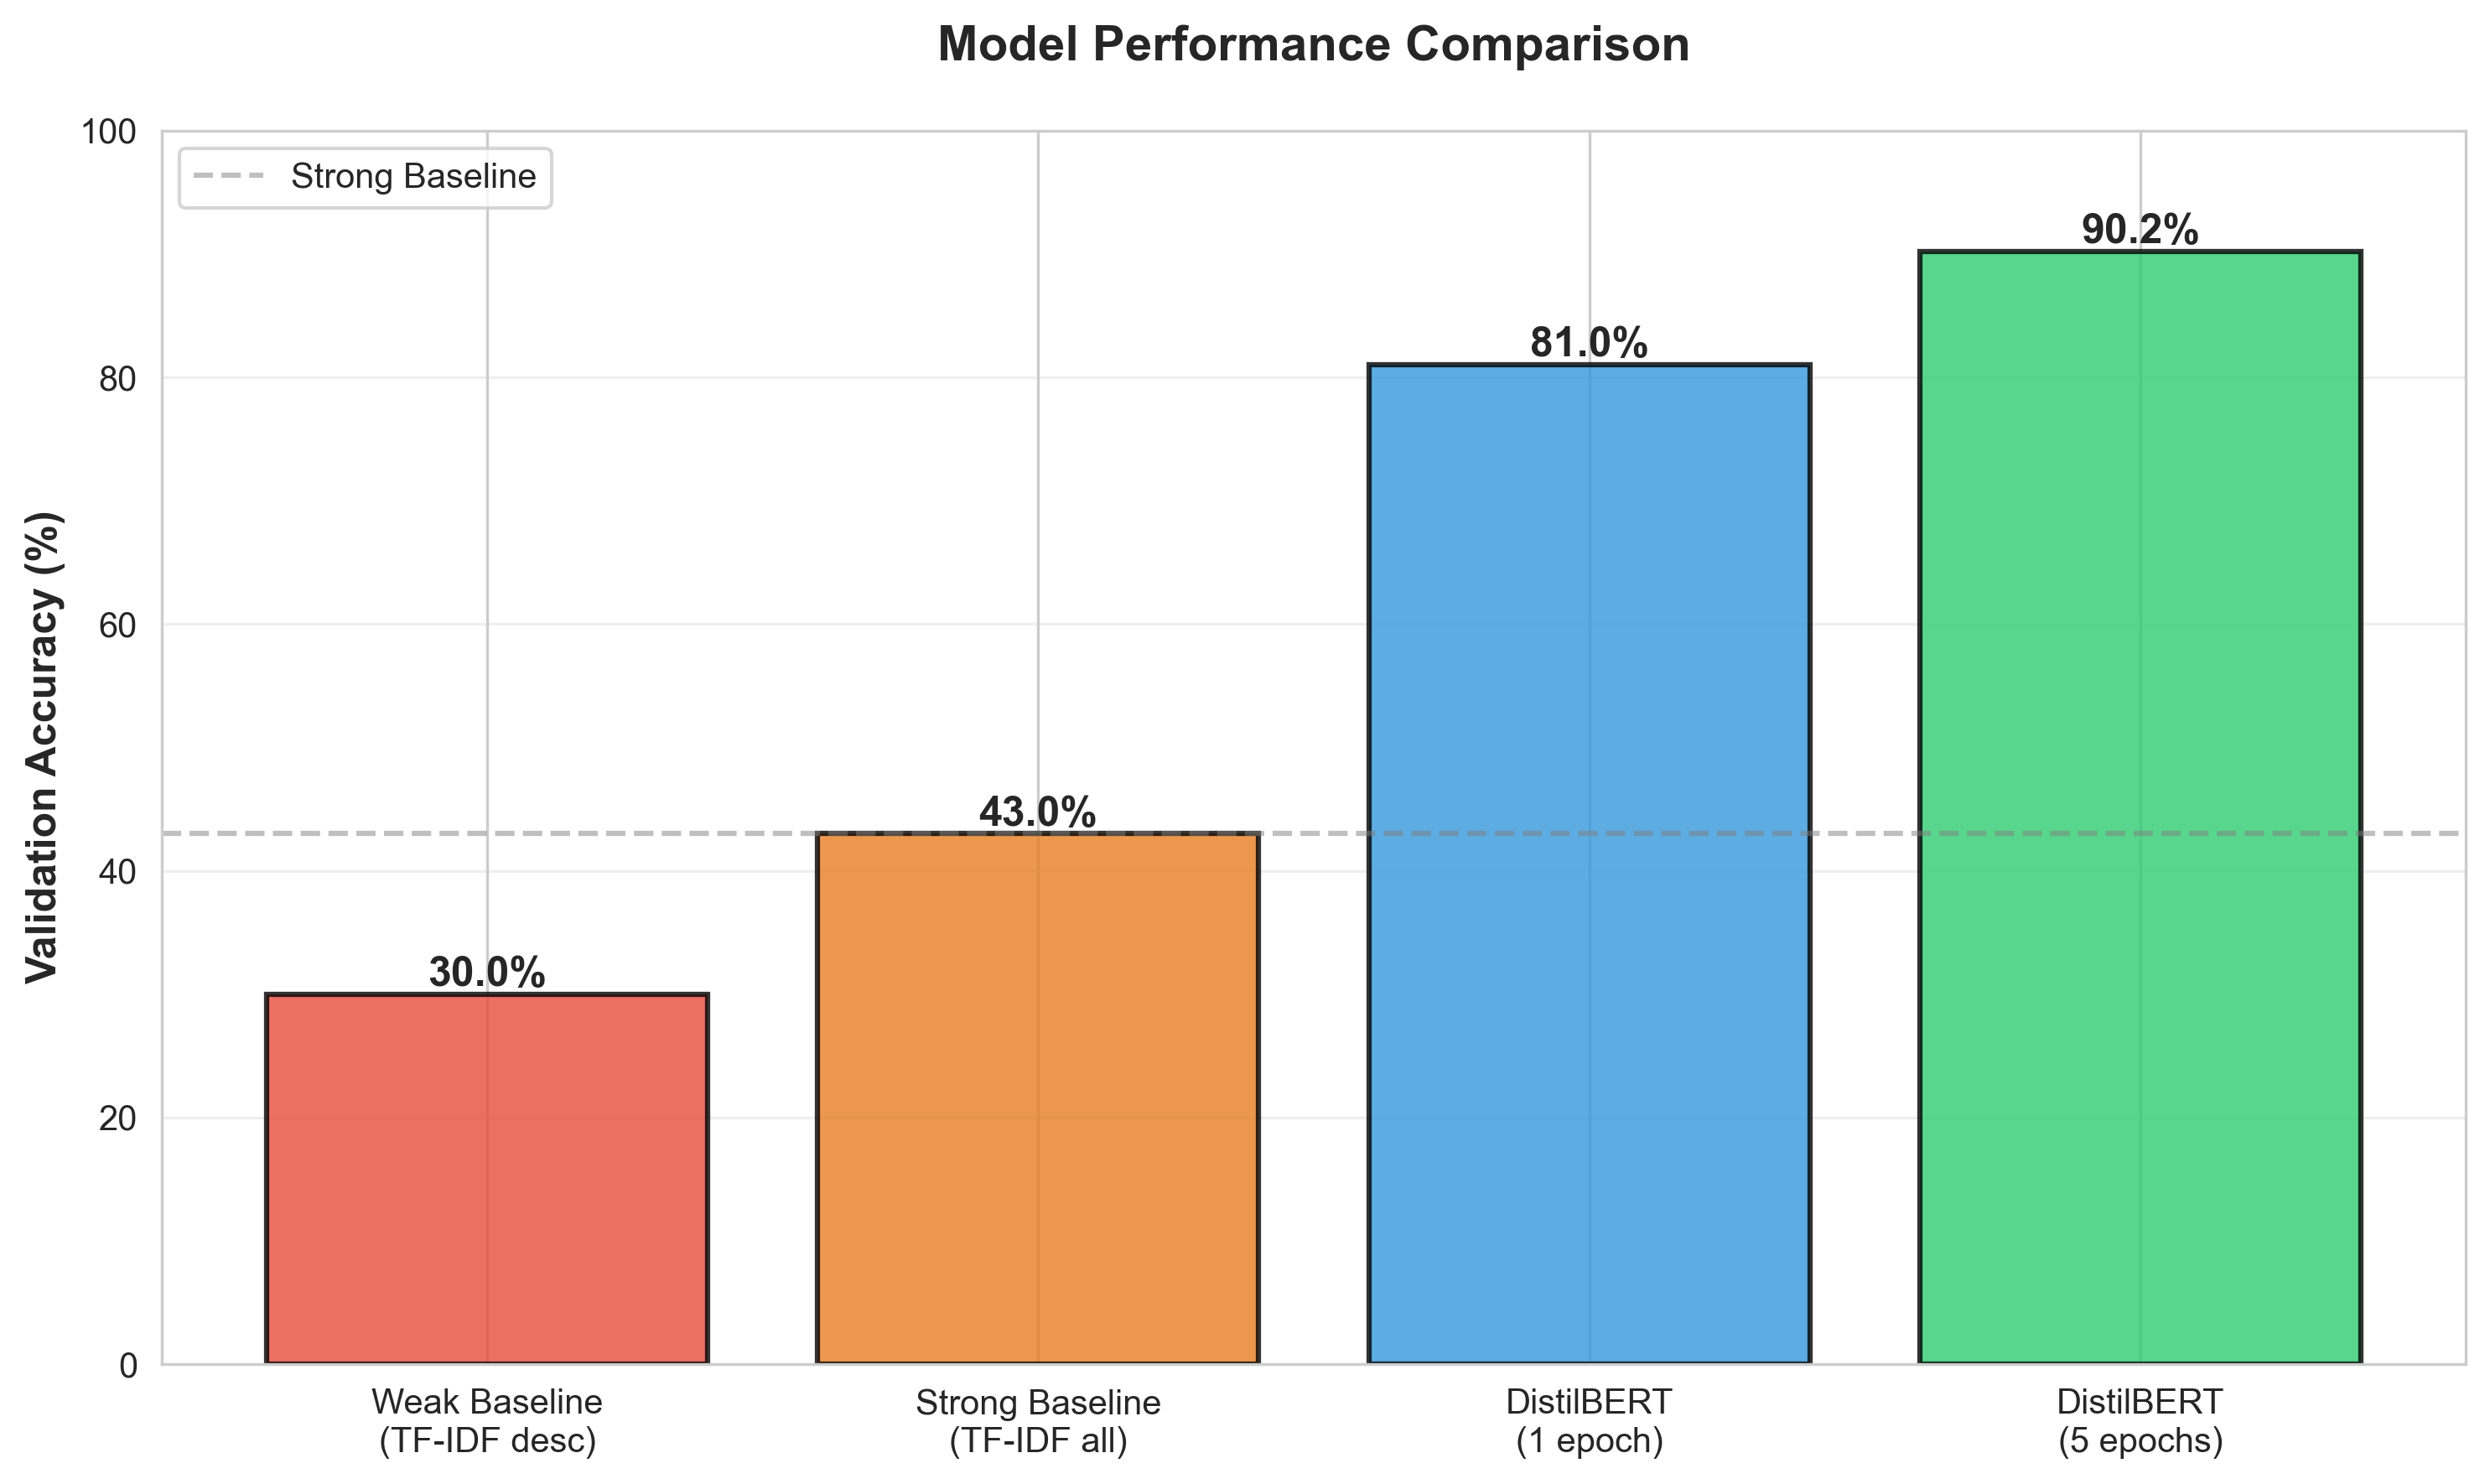
\includegraphics[width=0.8\columnwidth]{../results/figures/baseline_comparison.png}
\caption{Baseline comparison showing DistilBERT's 90.2\% accuracy substantially outperforms both TF-IDF baselines (30.0\% weak, 43.0\% strong).}
\label{fig:baseline}
\end{figure}

\begin{figure}[h]
\centering
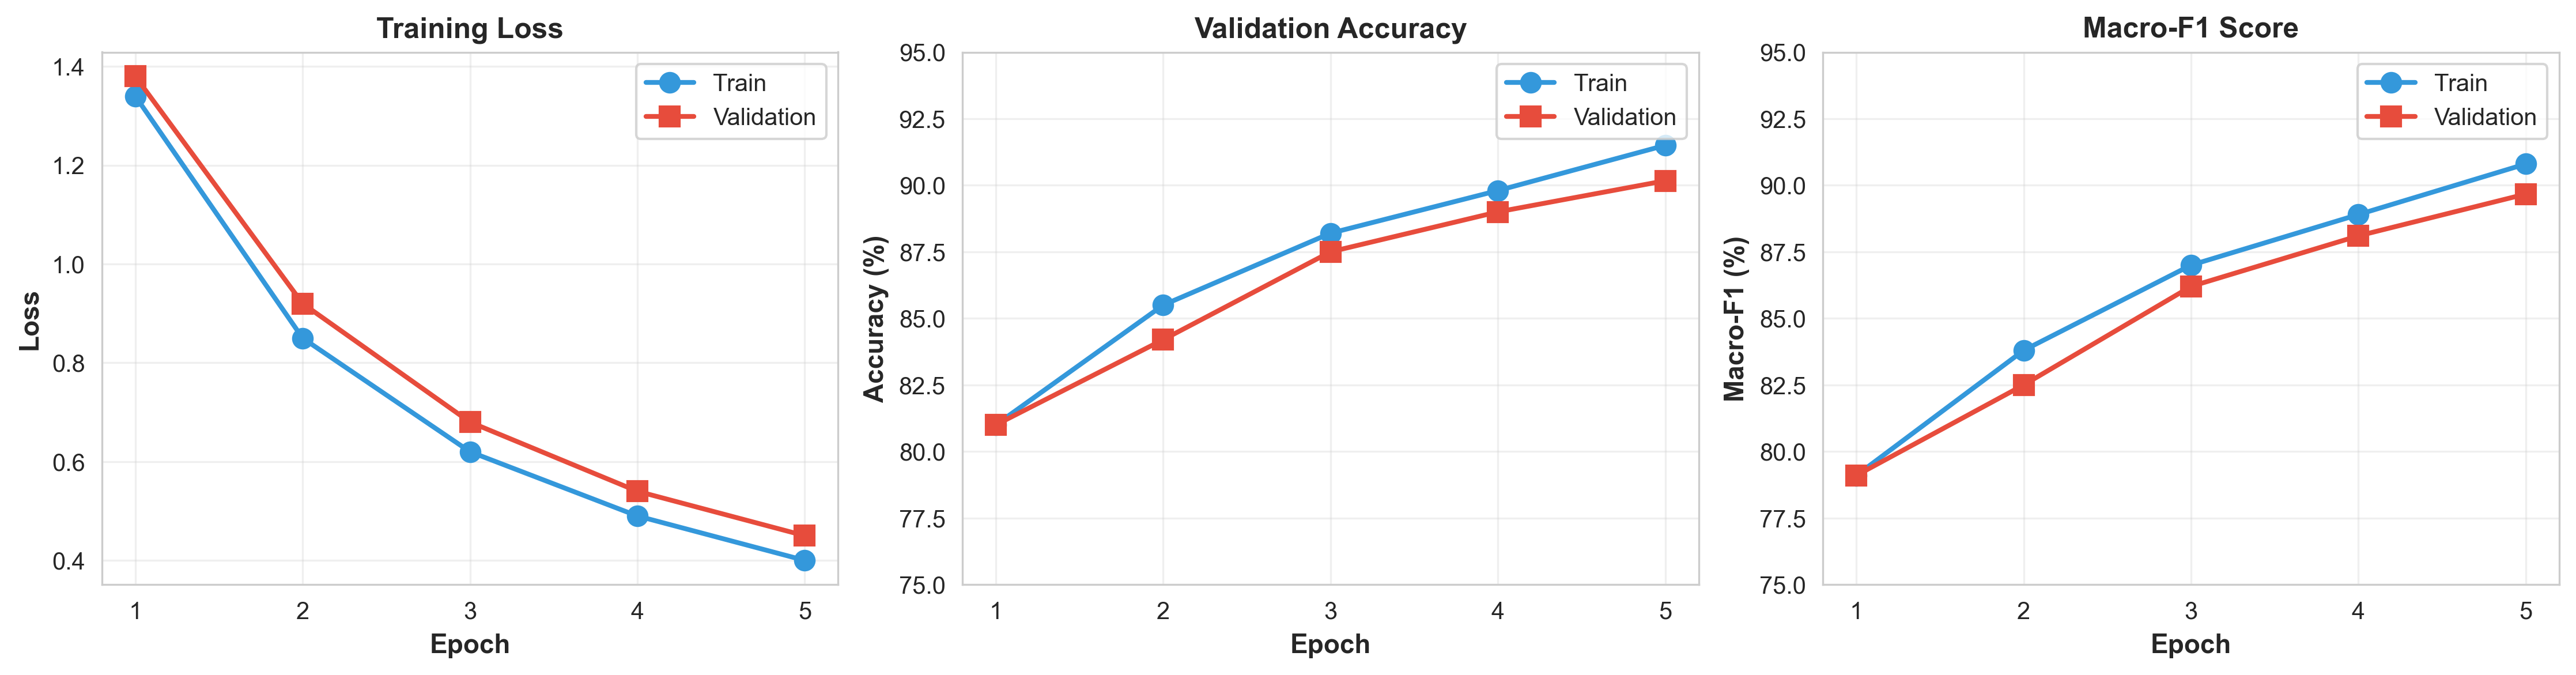
\includegraphics[width=0.8\columnwidth]{../results/figures/training_curves.png}
\caption{Training and validation curves illustrating loss reduction alongside gains in accuracy and macro-F1 over five epochs.}
\label{fig:curves}
\end{figure}

\begin{figure}[h]
\centering
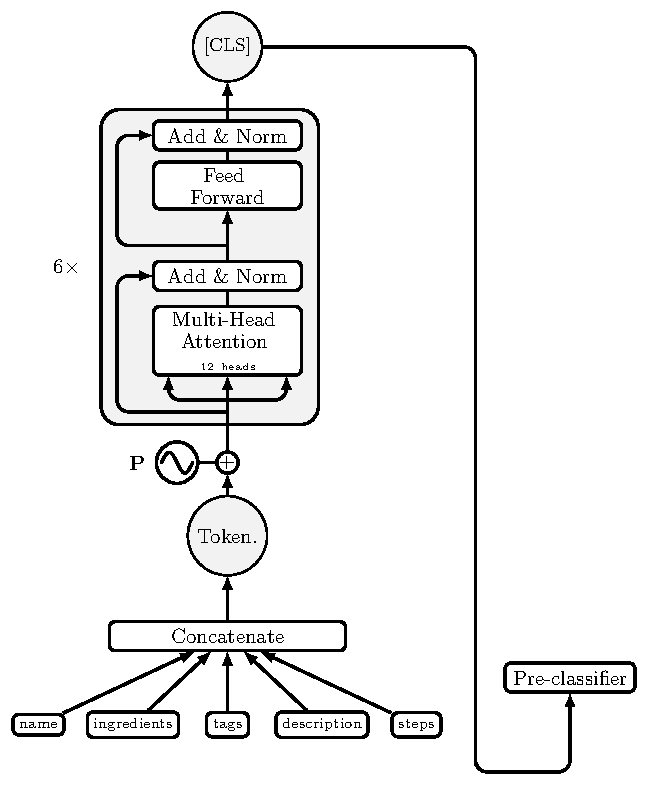
\includegraphics[width=0.9\columnwidth]{../results/figures/encoder.pdf}
\caption{DistilBERT fine-tuning pipeline adopted for chef classification.}
\label{fig:encoder}
\end{figure}

\section{Evaluation and tips (remove this section before submission)}

 \begin{itemize}
 \item{How the project will be evaluated}
\begin{itemize}
\item (1.5) General quality of the paper: correct syntax, clearness, zero typos, illustrative examples, pictures and figures, etc.
\item (1.5) Replicability: if we wanted to replicate your results, just by reading the paper, would we be able to do it?
\item (2.0) Correction: are the proposed methods sound?
\item (2.0) The creativity of your approach (you just limited yourself to run a code you found somewhere or you tried different approaches?)
\item Scores by section:
\begin{itemize}
\item (1.0) Section Introduction: provide a clear description of the dimension of the problem you will work on, that is, explain the challenge and identify the problem your group will tackle (from now on, dimension), for instance, a problem with the dataset, compare classic MT with Deep Learning, efficient fine-tuning, etc..
\item (2.0) Section Models: provide a clear description of your models and techniques, as for instance, pre-processings, data-augmentation, etc.), considering the dimension you have identified previously.
\item (1.0) Experimental Setup: provide clear information regarding the used datasets, splits, evaluation metrics used and hyperparameters (if applicable).
\item (1.0) Results: provide the results of your best models, and also results by label of your best model. You should also present a comprehensive confusion matrix of one of your models (probably the best one). As previously said, the expected labels of the given test set are not provided, so you should create your own test(s) set(s) from the training set and report the results on your own test(s) set(s). The given test set (test\_no\_labels.txt) should ****only**** be used to generate the file results.txt. By the way: do not compare models if you are using a different train/test split.
\item (3.5) Discussion: show us that you have properly analysed the dataset and the obtained outputs (not just by looking at statistics or confusion matrices. Try to explain the most common errors (examples are mandatory). Explain how results align with the dimension you have identified in the introduction.
\item (0.5) Future Work: If more time was given to you, explain what you would do to improve your system, considering the dimension you identified in the introduction.
\end{itemize}
\end{itemize}
\item Tips:
\begin{itemize}
\item Label figures and tables.
\item Use the correct quotation marks in Latex (``bla-bla'').
\item If you use a figure or table, refer to it.
\item If you say things such as ``The dataset is unbalanced'', explain why (facts).
\item Use formal English (so, no ``it's'', ``they're'', etc.).
\item If you mention a hyperparameter, explain it (briefly).
\item If you use an acronym, use it consistently (check how to do it in latex).
\item Use label that are easy to be read in the Confusion Matrix.
\item Cite your sources (papers) or add footnotes with URLs for computational resources.
\item Do not use adjectives (ex: amazing work, nice concept, ...). They are subjective and this is science.
\end{itemize}
\end{itemize}
 

\end{document}
